\chapter{Stabiliteitsberekening en maximale ladingmassa}
\label{chap:stabiliteit}

Voor de plaatsing van de zeezoutbatterijen in de centrale opslagruimte van
\emph{'t~Jansje} moet worden gecontroleerd of het schip in geladen conditie
nog voldoet aan de stabiliteitseisen en of de diepgang binnen de toegestane
grenzen blijft. Alle berekeningen zijn uitgevoerd voor zoetwater
($\rho = 1000\ \mathrm{kg/m^3}$), omdat \emph{'t~Jansje} voornamelijk vaart
op de Nieuwe Maas.

% ============================================================
\section{Scheepsgegevens en invoer}
\label{sec:stab_geometrie}

\begin{table}[H]
\centering
\caption{Invoerparameters stabiliteitsberekening}
\label{tab:stab_input}
\begin{tabular}{llll}
\toprule
Parameter & Symbool & Waarde & Eenheid \\
\midrule
\multicolumn{4}{l}{\textit{Scheepsgegevens}} \\
\midrule
Lengte waterlijn            & $L$      & 22{,}22 & m     \\
Maximale breedte            & $B$      &  4{,}36 & m     \\
Gemiddelde diepgang (leeg)  & $T$      &  1{,}50 & m     \\
Rompdiepte (kiel t/m dek)   & $D$      &  2{,}05 & m     \\
Verdringingsvolume (leeg)   & $\nabla$ & 73{,}0  & m$^3$ \\
Scheepsgewicht (leeg)       & $W$      & 73{,}0  & t     \\
Waterplancoëfficiënt        & $C_{WP}$ &  0{,}795& --    \\
\midrule
\multicolumn{4}{l}{\textit{Centrale opslagruimte}} \\
\midrule
Ruimlengte                  & $L_r$    &  3{,}00 & m     \\
Ruimbreedte                 & $B_r$    &  2{,}00 & m     \\
Ruimhoogte                  & $H_r$    &  2{,}00 & m     \\
\midrule
\multicolumn{4}{l}{\textit{Zeezoutbatterij -- per cel \cite{DrTenInfo2025}}} \\
\midrule
Massa per cel               & $m_b$    & 18{,}0  & kg    \\
Afmetingen ($l \times b \times h$) & -- & $0{,}39 \times 0{,}60 \times 0{,}23$ & m \\
Volume per cel              & $V_b$    & 0{,}0538& m$^3$ \\
\bottomrule
\end{tabular}
\end{table}

% ============================================================
\section{Batterijpakking}
\label{sec:batterijen}

Voordat de stabiliteit kan worden gecontroleerd, moet het aantal batterijen
dat in het ruim past worden bepaald. De gunstigste oriëntatie is met de
lange zijde (0{,}60~m) langs de ruimlengte:

\begin{equation}
    N_b = \left\lfloor \frac{3{,}00}{0{,}60} \right\rfloor \times
          \left\lfloor \frac{2{,}00}{0{,}39} \right\rfloor \times
          \left\lfloor \frac{2{,}00}{0{,}23} \right\rfloor
        = 5 \times 5 \times 8 = \boxed{200\ \text{cellen}}
    \label{eq:Nb}
\end{equation}

De totale ladingmassa en het volume bedragen:

\begin{align}
    M_\mathrm{bat} &= 200 \times 18{,}0\ \mathrm{kg} = \boxed{3{,}6\ \mathrm{t}}
    \label{eq:Mbat} \\[4pt]
    V_\mathrm{bat} &= 200 \times 0{,}0538 = 10{,}76\ \mathrm{m^3}
\end{align}

De pakkingsefficiëntie bedraagt $10{,}76/12{,}0 = 89{,}7\%$ Figuur~\ref{fig:bat_pakking} toont de schematische pakking in zijaanzicht.

\begin{figure}[H]
\centering
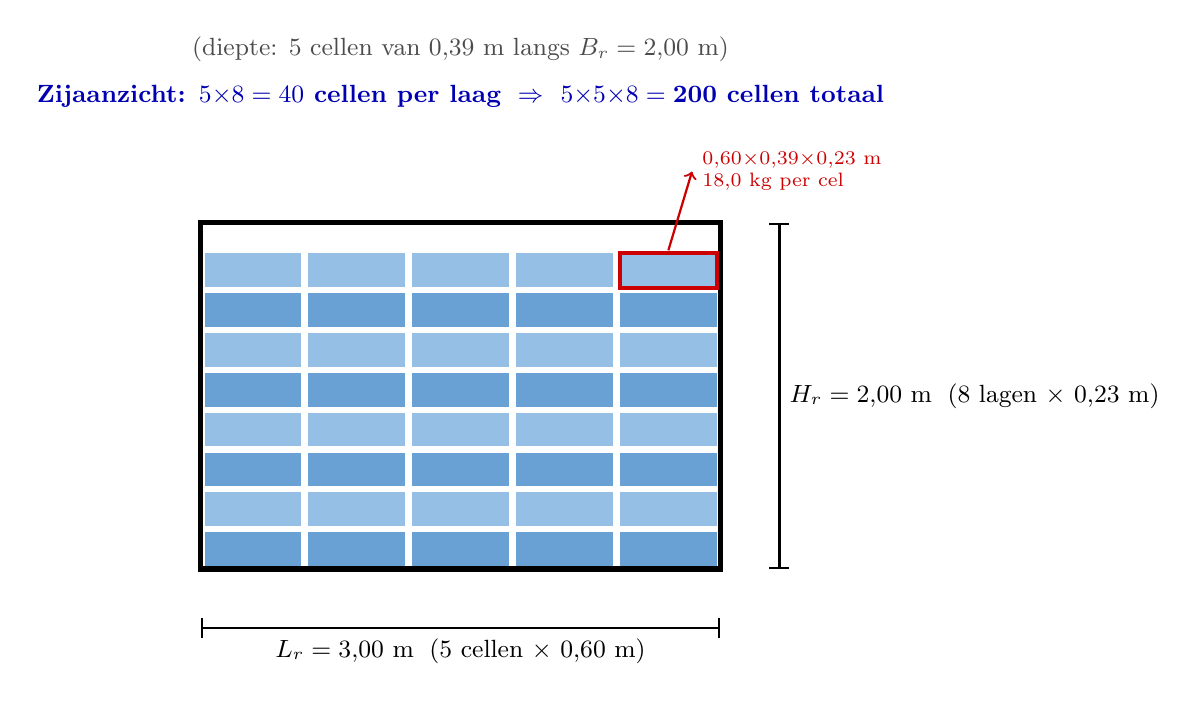
\begin{tikzpicture}
\def\sc{2.2}
\pgfmathsetmacro{\Lr}{3.00*\sc}
\pgfmathsetmacro{\Hr}{2.00*\sc}
\pgfmathsetmacro{\bl}{0.60*\sc}
\pgfmathsetmacro{\bh}{0.23*\sc}

\foreach \row in {0,...,7}{
    \foreach \col in {0,...,4}{
        \pgfmathsetmacro{\xpos}{\col*\bl}
        \pgfmathsetmacro{\ypos}{\row*\bh}
        \pgfmathparse{int(mod(\row,2))}
        \ifnum\pgfmathresult=0
            \definecolor{batcol}{RGB}{80,145,205}
        \else
            \definecolor{batcol}{RGB}{130,180,225}
        \fi
        \fill[batcol, opacity=0.85]
            (\xpos cm+0.04cm,\ypos cm+0.03cm)
            rectangle
            (\xpos cm+\bl cm-0.04cm,\ypos cm+\bh cm-0.03cm);
        \draw[white, line width=0.5pt]
            (\xpos cm+0.04cm,\ypos cm+0.03cm)
            rectangle
            (\xpos cm+\bl cm-0.04cm,\ypos cm+\bh cm-0.03cm);
    }
}
\draw[black, line width=2pt] (0,0) rectangle (\Lr cm,\Hr cm);

\draw[|-|, thick]
    (0,-0.75cm) -- (\Lr cm,-0.75cm)
    node[midway, below, font=\small]
        {$L_r = 3{,}00$~m \;(5 cellen $\times$ 0{,}60~m)};
\draw[|-|, thick]
    (\Lr cm+0.75cm,0) -- (\Lr cm+0.75cm,\Hr cm)
    node[midway, right, font=\small]
        {$H_r = 2{,}00$~m \;(8 lagen $\times$ 0{,}23~m)};

\pgfmathsetmacro{\hx}{4*\bl}
\pgfmathsetmacro{\hy}{7*\bh}
\draw[red!80!black, line width=1.4pt]
    (\hx cm+0.04cm,\hy cm+0.03cm)
    rectangle
    (\hx cm+\bl cm-0.04cm,\hy cm+\bh cm-0.03cm);
\draw[->, red!80!black, thick]
    (\hx cm+\bl cm*0.5,\hy cm+\bh cm)
    -- ++(0.3cm,1.0cm)
    node[right, font=\scriptsize, red!80!black, align=left]
        {$0{,}60{\times}0{,}39{\times}0{,}23$~m\\18{,}0~kg per cel};

\node[font=\small\bfseries, text=blue!70!black, align=center]
    at (\Lr cm*0.5,\Hr cm+1.6cm)
    {Zijaanzicht: $5{\times}8=40$ cellen per laag
     $\;\Rightarrow\;$ $5{\times}5{\times}8=\mathbf{200}$ cellen totaal};
\node[font=\small, text=gray!60!black, align=center]
    at (\Lr cm*0.5,\Hr cm+2.2cm)
    {(diepte: 5 cellen van 0{,}39~m langs $B_r=2{,}00$~m)};
\end{tikzpicture}
\caption{Pakking van de zeezoutbatterijen in het laadruim (zijaanzicht,
         $3{,}00 \times 2{,}00$~m). In de breedterichting passen 5 cellen
         van 0{,}39~m; totaal $5 \times 5 \times 8 = 200$ cellen
         \cite{DrTenInfo2025}.}
\label{fig:bat_pakking}
\end{figure}

% ============================================================
\section{Stabiliteitsberekening}
\label{sec:stab_berekening}

De initiële dwarsscheepse stabiliteit wordt bepaald door de metacentrische
hoogte \cite[p.~44]{Barras2006}:

\begin{equation}
    GM = KB + BM - KG \geq 0{,}15\ \mathrm{m}
    \label{eq:GM}
\end{equation}

\subsection{Lege conditie}

\paragraph{Hoogte drijfpunt $KB$}
Voor scheepsvormige vaartuigen geldt $KB \approx 0{,}535 \times T$
\cite[p.~104]{Barras2006}:

\begin{equation}
    KB = 0{,}535 \times 1{,}50 = 0{,}803\ \mathrm{m}
\end{equation}

\paragraph{Metacentrische straal $BM$}
Het tweede moment van het waterplan wordt benaderd via
\cite[Hfst.~1]{Schneekluth1998}:

\begin{equation}
    I_T = \frac{L\,B^3}{12}\!\left(0{,}096 + 0{,}89\,C_{WP}^2\right)
        = \frac{22{,}22 \times 4{,}36^3}{12}
          \!\left(0{,}096 + 0{,}89 \times 0{,}795^2\right)
        = 101{,}1\ \mathrm{m^4}
\end{equation}

\begin{equation}
    BM = \frac{I_T}{\nabla} = \frac{101{,}1}{73{,}0} = 1{,}384\ \mathrm{m}
    \qquad \cite[p.~107]{Barras2006}
\end{equation}

\paragraph{Zwaartepunt $KG$}
Voor \emph{'t~Jansje} is geen hellingsproef  uitgevoerd, waardoor $KG$ niet
direct bekend is. Omdat $KG$ afhangt van hoe het gewicht van het schip
verdeeld is over de constructie, is er ook geen algemene formule om het te
berekenen uit de hoofdafmetingen alleen.

Om toch een uitspraak te kunnen doen over de stabiliteit, is in
Tabel~\ref{tab:KG_gevoeligheid} berekend hoe $GM$ verandert voor
verschillende waarden van $KG$. Hieruit blijkt dat $GM$ pas onder het
IMO-minimum van 0{,}15~m zakt bij $KG > 2{,}04$~m. Dat is vrijwel gelijk
aan de rompdiepte ($D = 2{,}05$~m), wat fysisch onmogelijk is: het
zwaartepunt van het schip kan nooit hoger liggen dan het dek. Het schip
voldoet dus aan de stabiliteitseis voor elke realistische massaverdeling.
Voor de verdere berekening wordt $KG_\mathrm{leeg} = 1{,}30$~m aangehouden.

\begin{table}[H]
\centering
\caption{Gevoeligheid van $GM_\mathrm{leeg}$ voor de aanname van $KG$
         ($KM = KB + BM = 2{,}187$~m)}
\label{tab:KG_gevoeligheid}
\small
\begin{tabular}{ccc}
\toprule
$KG_\mathrm{leeg}$ [m] & $GM_\mathrm{leeg}$ [m] & Beoordeling \\
\midrule
1{,}00 & 1{,}187 & Ruim voldoende \\
1{,}10 & 1{,}087 & Ruim voldoende \\
1{,}20 & 0{,}987 & Ruim voldoende \\
\rowcolor{yellow!20}
1{,}30 & 0{,}887 & Ruim voldoende \\
1{,}50 & 0{,}687 & Voldoende \\
1{,}70 & 0{,}487 & Voldoende \\
1{,}90 & 0{,}287 & Voldoende \\
2{,}04 & 0{,}147 & Grenswaarde ($\approx$ IMO-minimum) \\
\bottomrule
\end{tabular}
\vspace{4pt}

\noindent\footnotesize
\textit{Gele rij: gehanteerde rekenwaarde. IMO-minimum: $GM \geq 0{,}15$~m.}
\end{table}

De metacentrische hoogte in lege conditie bedraagt daarmee:

\begin{equation}
    GM_\mathrm{leeg} = 0{,}803 + 1{,}384 - 1{,}30 = \boxed{0{,}887\ \mathrm{m}}
    \label{eq:GM_leeg}
\end{equation}

\subsection{Geladen conditie -- 200 batterijen (3{,}6~t)}

Het zwaartepunt van de lading wordt aangenomen op $z_b = 1{,}20$~m boven
kiel (ruimbodem op $\approx 0{,}20$~m, midden van de 2{,}00~m stapelhoogte
op $+1{,}00$~m). De nieuwe diepgang, het verdringingsvolume en de
stabiliteitgrootheden worden als volgt berekend:

\begin{align}
    A_{WP}              &= C_{WP} \cdot L \cdot B
                         = 0{,}795 \times 22{,}22 \times 4{,}36
                         = 77{,}0\ \mathrm{m^2} \\[4pt]
    T_\mathrm{gel}      &= 1{,}500 + \frac{3{,}6}{77{,}0}
                         = 1{,}547\ \mathrm{m}
                         \quad\Rightarrow\quad
                         \text{vrijboord} = 2{,}05 - 1{,}547 = 0{,}503\ \mathrm{m}
                         \\[4pt]
    \nabla_\mathrm{gel} &= 73{,}0 + 3{,}6 = 76{,}6\ \mathrm{m^3} \\[4pt]
    KB_\mathrm{gel}     &= 0{,}535 \times 1{,}547 = 0{,}828\ \mathrm{m} \\[4pt]
    BM_\mathrm{gel}     &= \frac{101{,}1}{76{,}6}  = 1{,}319\ \mathrm{m} \\[4pt]
    KG_\mathrm{gel}     &= \frac{73{,}0 \times 1{,}30 + 3{,}6 \times 1{,}20}
                               {76{,}6}
                         = \frac{94{,}90 + 4{,}32}{76{,}6}
                         = 1{,}296\ \mathrm{m} \\[4pt]
    GM_\mathrm{gel}     &= 0{,}828 + 1{,}319 - 1{,}296
                         = \boxed{0{,}851\ \mathrm{m}}
\end{align}

Beide criteria zijn gehaald: het vrijboord van 0{,}503~m ligt
 boven het minimum van 0{,}20~m, en $GM = 0{,}851$~m is
groter dan het IMO minimum van 0{,}15~m.

\subsection{Maximale toelaatbare ladingmassa}

Voor de volledigheid wordt ook de maximale bovengrens bepaald. 

De maximale diepgang is $T_\mathrm{max} = D - 0{,}20 = 1{,}85$~m,
zodat het schip nog $\Delta T = 1{,}85 - 1{,}50 = 0{,}35$~m mag inzakken.
Het gewicht van het daarmee extra verplaatste water geeft de maximale
ladingmassa:

\begin{equation}
    M_\mathrm{max} = \Delta T \times \rho \cdot A_{WP}
                   = 0{,}35 \times 1000 \times 77{,}0 \times 10^{-3}
                   = \boxed{27{,}0\ \mathrm{t}}
    \label{eq:Mmax}
\end{equation}

Bij deze massa is het $GM$ nog $0{,}779$~m (zie Figuur~\ref{fig:GM_vs_M}),
zodat de dwarsscheepse stabiliteit op geen enkel punt de beperkende factor is.
De werkelijke batterijlading van 3{,}6~t valt een factor 7{,}5 onder dit maximum.

\paragraph{Langsscheepse stabiliteit}
Het tweede moment om de dwarsscheepse as bedraagt
$I_L = C_{WP} \cdot BL^3/12 = 3169\ \mathrm{m^4}$, wat een langsscheepse
metacentrische hoogte geeft van:

\begin{equation}
    GM_L = KB + \frac{I_L}{\nabla} - KG
         = 0{,}803 + 43{,}4 - 1{,}30
         = 42{,}9\ \mathrm{m}
\end{equation}

Dit is een factor $\sim 48$ groter dan de dwarsscheepse $GM$ en is voor een
centraal geplaatste lading niet de beperkende factor.

% ============================================================
\section{Figuren}
\label{sec:stab_figuren}

\begin{figure}[H]
\centering
\begin{tikzpicture}[
    >=Stealth, scale=2.2,
    punkt/.style={circle, fill=#1, draw=#1!70!black, inner sep=2.2pt},
    lbl/.style={font=\small\bfseries, text=#1}
]
\def\Bhalf{2.0}
\def\D{2.05}
\def\T{1.50}
\def\KB{0.803}
\def\KG{1.300}
\def\KM{2.187}

\fill[blue!12] (-\Bhalf-0.3,0) rectangle (\Bhalf+0.3,\T);
\fill[blue!28, opacity=0.7] (-\Bhalf,0) rectangle (\Bhalf,\T);
\draw[blue!60!black, dashed, semithick]
    (-\Bhalf-0.4,\T) -- (\Bhalf+0.4,\T)
    node[right, font=\tiny, text=blue!70!black] {WL};
\draw[black, line width=1.6pt]
    (-\Bhalf,\D) -- (-\Bhalf,0) -- (\Bhalf,0) -- (\Bhalf,\D);
\draw[gray!40, thin, dashed] (0,-0.18) -- (0,2.55);

\node[punkt=black!80]       at (0,0)    {};
\node[punkt=blue!70!black]  at (0,\KB)  {};
\node[punkt=red!75!black]   at (0,\KG)  {};
\node[punkt=green!55!black] at (0,\KM)  {};

\node[lbl=black,           anchor=east] at (-0.10,0)    {$K$};
\node[lbl=blue!70!black,   anchor=east] at (-0.10,\KB)  {$B$};
\node[lbl=red!75!black,    anchor=east] at (-0.10,\KG)  {$G$};
\node[lbl=green!55!black,  anchor=east] at (-0.10,\KM)  {$M$};

\node[font=\tiny, text=blue!70!black,  anchor=west] at (0.08,\KB) {0{,}803~m};
\node[font=\tiny, text=red!75!black,   anchor=west] at (0.08,\KG) {1{,}300~m};
\node[font=\tiny, text=green!55!black, anchor=west] at (0.08,\KM) {2{,}187~m};

\draw[<->, thick, blue!60!black]
    (-0.65,0) -- (-0.65,\KB)
    node[midway, left, font=\scriptsize, text=blue!60!black] {$KB=0{,}803$~m};
\draw[<->, thick, orange!80!black]
    (-0.65,\KB) -- (-0.65,\KM)
    node[midway, left, font=\scriptsize, text=orange!80!black] {$BM=1{,}384$~m};
\draw[<->, thick, purple!80!black]
    (0.62,\KB) -- (0.62,\KG)
    node[midway, right, font=\scriptsize, text=purple!80!black] {$BG=0{,}497$~m};
\draw[<->, thick, green!55!black]
    (0.62,\KG) -- (0.62,\KM)
    node[midway, right, font=\scriptsize, text=green!55!black] {$GM=0{,}887$~m};

\draw[<->] (-\Bhalf,-0.14) -- (\Bhalf,-0.14)
    node[midway, below, font=\scriptsize] {$B = 4{,}36$~m};
\draw[<->] (\Bhalf+0.32,0) -- (\Bhalf+0.32,\T)
    node[midway, right, font=\scriptsize] {$T=1{,}50$~m};
\draw[<->] (\Bhalf+0.55,0) -- (\Bhalf+0.55,\D)
    node[midway, right, font=\scriptsize] {$D=2{,}05$~m};
\end{tikzpicture}
\caption{Dwarsdoorsnede van \emph{'t~Jansje} in lege conditie
         ($KG = 1{,}30$~m als rekenwaarde). $GM = 0{,}887$~m.}
\label{fig:stab_dwarsdoorsnede_leeg}
\end{figure}

\begin{figure}[H]
\centering
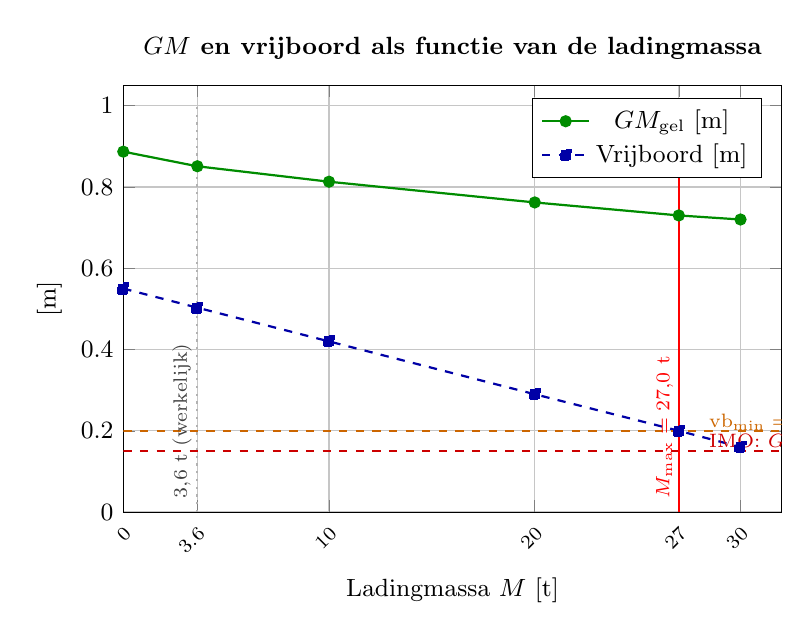
\begin{tikzpicture}
\begin{axis}[
    width=0.82\textwidth, height=7.0cm,
    xlabel={Ladingmassa $M$ [t]},
    ylabel={[m]},
    title={$GM$ en vrijboord als functie van de ladingmassa},
    xmin=0, xmax=32, ymin=0, ymax=1.05,
    xtick={0,3.6,10,20,27,30},
    xticklabel style={font=\scriptsize, rotate=45, anchor=north east},
    grid=both,
    grid style={line width=0.3pt, draw=gray!25},
    major grid style={line width=0.5pt, draw=gray!45},
    legend pos=north east, legend style={font=\small},
    tick label style={font=\small}, label style={font=\small},
    title style={font=\small\bfseries},
]
\addplot[green!55!black, thick, mark=*, mark size=1.8pt] coordinates {
    (0,0.887)(3.6,0.851)(10,0.813)(20,0.762)(27,0.730)(30,0.720)
};
\addlegendentry{$GM_\mathrm{gel}$ [m]}

\addplot[blue!65!black, thick, dashed, mark=square*, mark size=1.8pt] coordinates {
    (0,0.550)(3.6,0.503)(10,0.420)(20,0.290)(27,0.200)(30,0.160)
};
\addlegendentry{Vrijboord [m]}

\addplot[red!80!black, dashed, thick, forget plot]
    coordinates {(0,0.15)(32,0.15)};
\node[red!80!black, font=\scriptsize, anchor=west]
    at (axis cs:28,0.17) {IMO: $GM \geq 0{,}15$~m};

\addplot[orange!80!black, dashed, thick, forget plot]
    coordinates {(0,0.20)(32,0.20)};
\node[orange!80!black, font=\scriptsize, anchor=west]
    at (axis cs:28,0.22) {vb$_\mathrm{min}=0{,}20$~m};

\addplot[red, thick, forget plot] coordinates {(27,0)(27,1.0)};
\node[red, font=\scriptsize, rotate=90, anchor=south west]
    at (axis cs:27.2,0.01) {$M_\mathrm{max}=27{,}0$~t};

\addplot[gray!60, thick, dotted, forget plot] coordinates {(3.6,0)(3.6,1.0)};
\node[gray!50!black, font=\scriptsize, rotate=90, anchor=south west]
    at (axis cs:3.8,0.01) {3{,}6~t (werkelijk)};
\end{axis}
\end{tikzpicture}
\caption{$GM$ en vrijboord als functie van de ladingmassa ($KG_\mathrm{leeg}
         = 1{,}30$~m). De rode verticale lijn markeert de vrijboordlimiet
         van 27{,}0~t. De werkelijke batterijlading van 3{,}6~t valt ver
         binnen beide criteria.}
\label{fig:GM_vs_M}
\end{figure}

% ============================================================
\section{Overzicht resultaten}
\label{sec:stab_overzicht}

\begin{table}[H]
\centering
\caption{Stabiliteitsoverzicht \emph{'t~Jansje} -- lege en geladen conditie}
\label{tab:stab_overzicht}
\begin{tabular}{lrrl}
\toprule
Grootheid & Leeg & Geladen ($3{,}6$~t) & Eenheid \\
\midrule
Diepgang $T$             & 1{,}500 & 1{,}547 & m     \\
Vrijboord                & 0{,}550 & 0{,}503 & m     \\
$\nabla$                 & 73{,}0  & 76{,}6  & m$^3$ \\
\midrule
$KB$                     & 0{,}803 & 0{,}828 & m \\
$BM$                     & 1{,}384 & 1{,}319 & m \\
$KG$                     & 1{,}300 & 1{,}296 & m \\
\midrule
\rowcolor{green!15}
$GM$                     & \textbf{0{,}887} & \textbf{0{,}851} & m \\
IMO-minimum $GM$         & \multicolumn{2}{c}{0{,}150} & m \\
CCR-minimum $GM$ \cite{CCR2015} & \multicolumn{2}{c}{0{,}300} & m \\
\bottomrule
\end{tabular}
\end{table}

% ============================================================
\section{Beperkingen}
\label{sec:stab_beperkingen}

\begin{itemize}
    \item \textbf{$KG$-schatting}: Er is geen hellingsbroef gedaan met Jansje,
          waardoor $KG$ niet bekend is. Uit
          Tabel~\ref{tab:KG_gevoeligheid} blijkt echter dat $GM$ pas onder
          het IMO minimum zakt bij $KG > 2{,}04$~m. Omdat het dek op
          2{,}05~m zit, is dit onmogelijk. Onze conclusie over de stabiliteit klopt dus ,ongeacht de werkelijke waarde van $KG$.

    \item \textbf{Vrijboordmarge}: De minimale marge van 0{,}20~m is
          conservatief aangenomen. De exacte eis volgt uit de ES-TRIN/CCR
          regelgeving.

    \item \textbf{Grote hellingshoeken}: $GM$ beschrijft uitsluitend de
         stabiliteit voor kleine hellingshoeken ($\phi < 10^\circ$). Voor een volledig
          stabiliteitsoordeel is een $GZ$-diagram vereist
          \cite[p.~134]{Barras2006}.
\end{itemize}

% ============================================================
\section*{Conclusie}
\label{sec:stab_conclusie}

In de centrale opslagruimte passen geometrisch $\mathbf{200}$
zeezoutbatterijcellen ($M_\mathrm{bat} = \mathbf{3{,}6}$~t). De
metacentrische hoogte neemt af van $0{,}887$~m (leeg) naar $0{,}851$~m
(geladen), dit is boven het IMO minimum van $0{,}15$~m. Het vrijboord van 0{,}503~m in geladen conditie
is ook voldoende. De maximaal toelaatbare ladingmassa bedraagt
$27{,}0$~t; de werkelijke batterijlading valt daar een factor $7{,}5$
onder.